\documentclass{article}
\usepackage[left=0.85in, right=0.85in, top=0.5in, bottom=0.95in]{geometry}
\usepackage[T1]{fontenc}
\usepackage[utf8]{inputenc}
\usepackage[italian]{babel}
\usepackage{pdfpages}
\usepackage{graphicx}
\usepackage{wrapfig2}
\usepackage{amsmath}
\usepackage{amsthm}
\usepackage{amssymb}
\usepackage{cases}
\usepackage{gensymb} %simboli come ° = \degree  etc etc
\usepackage{subcaption}
\usepackage{hyperref}
\hypersetup{
	colorlinks=true,
	linkcolor=blue,    
	urlcolor=blue,
	%pdfpagemode=FullScreen,
}
\urlstyle{same}
\usepackage{changepage}
\usepackage{lastpage, epstopdf}
\usepackage{fancyhdr}
\usepackage{tcolorbox}
\usepackage{background}
\usepackage{tikz}
\usetikzlibrary{patterns}


%=======HEADER & FOOTER=======%
\def\lesson{Lezione N. 13}
\def\outcome{\textbf{Learning Outcomes:} Outcomes go here. }

\pagestyle{fancy}
\fancyhf{}
\renewcommand{\headrulewidth}{0pt}
\renewcommand{\footrulewidth}{1.4pt}
\lfoot{A.M. $\diamond$ \the\year}
\cfoot{Page \thepage}
\rfoot{\lesson}

%=======CORNELL STYLE FORMAT=======%
\SetBgScale{1}
\SetBgAngle{0}
\SetBgColor{black}
\SetBgContents{\rule{1pt}{0.85\paperheight}}
\SetBgHshift{-1.6in}
\SetBgVshift{-0.1in}

%=======CUSTOM BOXES=======%

\parindent 0ex

%=======BODY=======%
\begin{document}
	\setcounterpageref{secnumdepth}{0}
	\section*{Parte 9} %Date: \hrulefill}
%	\begin{tcolorbox}{\outcome}\end{tcolorbox}

\begin{adjustwidth}{2in}{} 
	
\textbf{{\Large Coefficiente di
		sicurezza e affidabilità}} \mbox{} \newline
		Con questa parte si chiuderà la trattazione del processo di verifica di un componente meccanico. \newline
		
		È stato trattato come una verifica strutturale prevedesse una riscontro fra una grandezza di progetto, questa derivante da condizioni di lavoro, e una grandezza di riferimento considerata ammissibile. 		
		\[\sigma_{eq}\leq \sigma_{amm}\]		
		Il termine a destra $\sigma_{amm}$ non è però direttamente derivante dalla prova di caratterizzazione del materiale ma è un valore considerato ammissibile tenuto conto di un opportuno margine di sicurezza. \newline
		
		Si introduce infatti un vero e proprio \textbf{coefficiente di sicurezza $X$}, scalare, che andando a dividere la resistenza del materiale ottenuta in laboratorio abbasserà il termine di confronto, portando da una tensione limite ad essere una tensione ammissibile. \newline
		
		Questo coefficiente di sicurezza nasce proprio per tenere in considerazione tutte quelle incertezze che si avevano sia nell'ambito della caratterizzazione e della qualità del materiale, sia per quanto riguarda i modelli descrittivi disponibili, questi, finché la geometria era semplice erano sufficientemente affidabili, e a seconda delle capacità di calcolo e delle teorie a disposizione si potevano avere fattori di sicurezza pari a 20, 30, \dots, va da se però che un coefficiente così valutato porta ad un calcolo poco ottimizzato, perché se da un lato metta al sicuro il  progettista da conseguenze legali legate a un cedimento eccezionale e accidentale del componente dovuto a carichi\textit{off normal} non a progetto, dall'altro lato appesantisce il componente meccanico: usare un fattore di sicurezza 10 su una trave sottoposta a trazione vuol dire avere una sezione resistente  10 volte più grande, e quindi maggiori ingombri, peso e costi. 
	    
	    La scelta del giusto coefficiente  di sicurezza è un aspetto estremamente delicato: è un equilibrio che dev'essere ricercato dal progettista in conformità di tutta una serie di vincoli imposti da normative e committenti. \newline
	    
	    Il coefficiente di sicurezza si configura così come il rapporto tra una resistenza che si dice  \textit{significativa del materiale}, relativa cioè al processo di cedimento che si sta considerando (snervamento per materiale duttile, a fatica, a rottura per materiale fragile), e una  tensione \textit{significativa corrispondente} a quello specifico processo di cedimento considerato relativa a condizioni di carico operative: è il rapporto tra la tensione limite e la tensione effettiva applicata sul componente. 
	    \[X = \dfrac{\text{resistenza significativa del materiale}}{\text{tensione significativa corrispondente}} = {\sigma_{\text{limite}}\over\sigma_{eq}}\]
	    La $sigma_{eq}$ è la tensione equivalente monodimensionale ottenuta attraverso un opportuno criterio di resistenza. 
	    
	    La $ \sigma_{\text{limite}} $ è il valore limite del materiale ottenuto in condizioni nominali di laboratorio e studiato in condizioni standard (per garantire la ripetibilità); se tali condizioni standard non dovessero essere garantite sarà allora il coefficiente di sicurezza ad entrare in gioco per tutelare la conservatività del progetto. 
\newpage	    	 
	    Un'altra definizione del coefficiente di sicurezza è il rapporto secco tra il carico limite di progetto e il carico nominale, normale:
	    \[X = \dfrac{\text{carico limite di progetto}}{\text{carico normale}}\]
	    Questa definizione, che sembra ricalcare la precedente, ha però un significato più ampio, il coefficiente di sicurezza in questo modo non si configura più come un rapporto fra due grandezze corrispondenti. 
	    
	    L'esempio può essere fornito una sollecitazione di compressione su un'asta, il carico limite è rappresentato - per determinate dimensioni dell'asta - dal carico di compressione che porta a snervamento, si nota però che per determinati valori di snellezza dell'asta il carico limite improvvisamente cambia e la condizione più conservativa ricade non più sul carico, ma sull'instabilità della stessa: cambia il valore del coefficiente  di sicurezza. 
	    
	    Questa definizione prevede perciò al numeratore qualunque fenomeno porti alla rottura, al guasto, o al danneggiamento del componente e al denominatore il carico effettivo: questa più ampia definizione abbraccia contemporaneamente tutti i processi di cedimento possibili. \newline	    
	    
	    Se ci si limita ad una verifica di tipo statico (oggetto di questa trattazione), si parla allora di un coefficiente $ X $ che si applica alle tensioni presenti sul materiale, per cui la disuguaglianza affrontata all'inizio:
	    \[\sigma_{eq}\leq\sigma_{amm}\]
	    Diviene: 
	    \[\sigma_{eq}\leq{\sigma_{lim, lab, standard}\over X} = \sigma_{amm}\]
	    Il coefficiente di sicurezza contiene tutte le incertezze relative sia al termine di sinistra: \textit{che modello ho utilizzato per generare quella tensione equivalente? Era calzante o violava alcune delle ipotesi del modello analitico? I carichi sono perfettamente definiti o possono subire variazioni durante l'esercizio? }
	    
	    Che nel temine di destra: \textit{la tensione limite è relativa al campione di materiale preso dalla stessa partita spedita o è un valore di letteratura o di riferimento? Le dimensioni del provino erano standard? Era un provino proveniente dallo stesso banco di laminazione o preso da un altro campione di materiale non laminato? } \newline
	    
	    Lo stesso coefficiente si trova anche in alcune normative come le Norme Tecniche sulle Costruzioni (NTC) con il ruolo di amplificatore statistico dei carichi, piuttosto che limite sulla resistenza del materiale, in questo modo si introduce un'incertezza legata alla stima effettiva degli stessi carichi. Un esempio può essere dato dal fatto che le forze peso valutate in NTC vengono moltiplicate per un fattore $ 1.1\div1.3 $ legato al fatto che il carico sul solaio di una costruzione oltre ad avere un certo valore da considerare come peso delle stesse componenti possiede anche una variabilità di carichi gravanti sul solaio stesso. Si valuta perciò a normativa che magari il 30\% in più è un picco di questa variazione e quindi un 1.3 diviene un fattore di sicurezza accettabile.
	    
	    In questo modo la tensione limite non viene toccata ma viene considerata come riferimento. 
	    \[xP_{norm}\leq P_{\text{limite}}\]
\newpage
	    Il peso che ogni incertezza ha sull'effettiva validazione del calcolo viene consigliato da sia da normative di riferimento che regolano i valori da assegnare, come le ASME per i pressure vessel, come le NTC appena viste, gli EuroCodici, le normative armonizzate UNI-EN, \dots sia da accordi tra committente e il progettista.\newline
	    
	    Ma quali sono gli aspetti che gravano sulla scelta di questo coefficiente?
	    \begin{enumerate}
	    	\item Innanzitutto, il grado di incertezza sui carichi, questo deriva dalle condizioni di utilizzo del pezzo. Magari per un componente meccanico che lavora in condizioni controllate di carico il margine di sicurezza da considerare sarà molto basso, caso diverso se si sta dimensionando un componente di cui non si è in grado di sapere quali siano i carichi applicati (ex. sospensione autovettura): condizioni poco prevedibili portano ad una grande incertezza sui carichi, in quel caso si utilizzerà un coefficiente di sicurezza decisamente superiore. 
	    	
	    	\item Altro paramento è l'incertezza sulla resistenza del materiale, e questo dipenderà, come detto poco sopra, dal campionamento del materiale, dalla scelta del provino \dots
	    	
	    	\item C'è poi da considerare l'incertezza sulla correlazione tra i carichi applicati e la resistenza del materiale stesso, questo vuol dire sostanzialmente chiedersi se il modello utilizzato per ricavare lo stato tensionale sul componente è un modello affidabile. 
	    	
	    	Si sono utilizzati modelli dalle ipotesi molto forti rispetto al caso reale oppure il caso reale rispetta tutte le ipotesi fatte? Ci sono delle variabili che non sono state prese in considerazione nella modellazione? Si è in grado di ricavare la concertazione di tensione, di valutare effettivamente la distribuzione di tensione sulla geometria complessa in esame? 
	    	
	    	\item Saranno poi da considerare le conseguenza legate al cedimento e alla sicurezza del personale: più aumenta il rischio che il personale venga danneggiato e più i coefficienti di sicurezza saranno maggiori.
	    	
	    	\item Ci saranno infine valutazioni economiche, un alto coefficiente di sicurezza vuol dire tanto materiale, maggior costo e basse prestazioni. 
	    	
	    	Evitare un danno mediante l'utilizzo di un coefficiente di sicurezza può avere degli aspetti economici da dover valutare: è meglio avere un danno frequente ma riparabile a costi contenuti dato da un coefficiente di sicurezza basso e rischiare un danno all'immagine per quanto riguarda l'affidabilità, o è meglio aumentare il coefficiente di sicurezza e quindi diminuire la probabilità di danno ma aumentare il costo all'utente? 
	    	
	    	È migliore un componente tecnologicamente avanzato che lavora meglio ma si guasta dopo pochi anni, o un componente che lavora per molti anni ma tecnologicamente meno avanzato e che garantisce minori prestazioni?
	    	
	    	Dare un coefficiente di sicurezza che garantisca una durata di 20 anni del componente costa molto di più all'utente e non si riesce più a garantire in questo modo un prezzo finale concorrenziale.
	    \end{enumerate}
\newpage
	    Qual è  quindi il valore del coefficiente di sicurezza da utilizzare? Valori tipici sono:
	     \begin{itemize}
	     	\item 1.25÷1.5 per materiali eccezionalmente affidabili, in condizioni controllate e con un peso da dover contenete. In queste occasioni carichi e tensioni sono ricavabili con
	     	certezza: i modelli analitici di calcolo sono estremamente affidabili e calzano perfettamente il componente. 
	     	\item 1.5÷2 per materiali ben caratterizzati, in condizioni ambientali costanti, con carichi e tensioni ricavabili con
	     	certezza.
	     	\item 2÷2.5 per materiali di qualità media, in condizioni ordinarie con carichi e tensioni determinabili.
	     	\item 2.5÷3 per materiali poco caratterizzati o fragili, in condizioni ambientali, di carico e di tensione di
	     	media variabilità.
	     	\item 3÷4 per materiali non caratterizzati, con valore di targa, in condizioni ambientali e di carico e di tensione di media variabilità
	     	oppure per materiali caratterizzati ma in condizioni ambientali e di carico e di tensione di incerta valutazione.
	     \end{itemize}
     		
     	Per carichi ripetuti, come ad esempio la fatica, il coefficiente di sicurezza non viene più applicato alle tensioni di snervamento o rottura ma su una tensione ammissibile derivante dai limiti di durata del componente. 
     	
     	Se si sta verificando ad urto, gli stessi coefficienti si applicano a un'ammissibile ad urto, questa terrà conto della resilienza del materiale, ovvero della sua della capacità di deformarsi a seguito di impatto, di assorbire energia, 
     	
     	Per materiali fragili infine, proprio perché il raggiungimento di una tensione limite porta ad un istantaneo cedimento del componente, si utilizzeranno dei coefficiente raddoppiati rispetto ai materiali duttili. \newline 
     	
     	\textbf{\Large Affidabilità} \newline 
     	Quanto appena visto è un approccio deterministico largamente utilizzato per il primo dimensionamento di un componente, rappresenta tuttavia una limitazione di quello che è il suo reale comportamento in condizioni di lavoro vere. Nel dimensionamento di un processo, si metterà in conto nella fase di progettazione che una percentuale di componenti prodotti sia difettoso.
     	
     	Avere una $ TOT $ quantità di componenti a prima vista identici non porta ad avere la sicurezza che tutti i $ TOT $ componenti funzionino davvero, esisterà una certa quantità $ tot $ di componenti che si romperanno durante il funzionamento, eppure avevano tutti lo stesso margine di sicurezza e derivavano dalla stessa partita di materiale. 
     	
     	Questo fa capire come ad esempio la probabilità del 98\% di sopravvivenza di un componente significa che il problema va approcciato in modo più statistico che deterministico, infatti la distribuzione statistica di una grandezza relativa al componete avrà sempre una certa dispersione; dire che il componente è soggetto ad una determinata tensione nominale è un'idealizzazione, questa infatti può fluttuare in dipendenza di chissà quanti fattori. \newline
     	
     	Si limiti il problema ad una verifica statica.
     	Si ipotizzi il componente in esame soggetto ad una tensione media applicata $\mu_y$ di $ 40PMa $, questo vorrà dire che il restante campione di provini sarà distribuito attorno alla media con una distribuzione gaussiana, questa caratterizzata da simmetria intorno alla media e da una deviazione standard $\sigma_y$ indice della dispersione dei valore intorno alla media. 
     	
     	
     	Se si è ipotizzata l'esistenza di una gaussiana per il valore di tensione applicato sul componente si può ipotizzare una gaussiana anche per il valore di resistenza media del componente $\mu_x$, magari $ 70MPa $: c'è un fattore di sicurezza $\approx 1.7$ di mezzo, sufficientemente importante, ma è successo lo stesso che alcuni componenti si sono rotti: perché? 
     	
     	\begin{figure}[H]
     		\centering
     		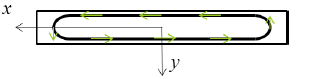
\includegraphics[width=0.5\linewidth]{immagini/screenshot006}
     		\label{fig:screenshot006}
     	\end{figure}
     	
     	Le code delle gaussiane si intersecano per un valore di tensione. L'area sottesa a questa intersezione rappresenta proprio la combinazione di provini particolarmente deboli (inclusioni nel materiale?) e molto sollecitati (fluttuazione del carico?) che porta a rottura quei $tot$ provini, il risultato è che quindi in quell'area la resistenza è inferiore al carico applicato. \newline
     	
     	Se questo concetto lo si esprime in funzione di una nuova grandezza chiamata margine di sicurezza $z$, essendo questa una funzione differenza tra i valori di resistenza e tensione e quindi una combinazione di due grandezze con distribuzione normale gaussiana, sarà anch'essa una distribuzione normale gaussiana caratterizzata da una media $\mu_z$ di $ 30MPa $. 
     	
     	\begin{figure}[H]
     		\centering
     		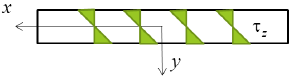
\includegraphics[width=0.5\linewidth]{immagini/screenshot007}
     		\label{fig:screenshot007}
     	\end{figure}
     	     	
     	In un grafico questa distribuzione si attesta intorno al suo valore medio e presenta una coda che raggiunge valori negativi: i casi caratterizzati da un margine di sicurezza negativo, sono quelli relativi ai componenti rotti, per cui la probabilità di rottura sarà legata alla coda al di là dello zero, che raggiunge valori negativi. 
     	
     	La distribuzione statistica gaussiana normale è definita come:
     	\[p(x) = \dfrac{1}{\sigma\sqrt{2\pi}}e^{-\dfrac{(x-\mu)^2}{2\sigma^2}} \] 
     	Con media $\mu$ e deviazione standard $\sigma$ rispettivamente pari a:
     	\[\mu = \sum_{i=1}^{n}{x_i\over n} \hspace{1cm} \sigma = 
     	\sqrt{\dfrac{\sum_{i=1}^{n}(x_i-\mu)^2}{n-1}}\]
     	La probabilità unitaria è data da: 
     	\[ \int_{-\infty}^{+\infty} p(x)dx = 1 = 100\%\]
     	Ed è l'area sottesa dalla gaussiana normalizzata. Per sapere qual è la probabilità di trovare un campione tra due ascisse distinte, si calcolerà il rispettivo integrale:
     	\[\int_{x_1}^{x_2} p(x)dx\]
     	La probabilità di rottura del caso precedente diviene così rappresentata dall'area sottesa al grafico per valori negativi. 
     	
     	In base alla distribuzione di $\sigma$ si ha una probabilità di avere un campione all'interno  della gaussiana. Il rage intorno al valore medio di $\pm\sigma$ porta ad avere una probabilità del 68\%, per $\pm2\sigma$ del 98\% e così via.
     	
     	\begin{figure}[H]
     		\centering
     		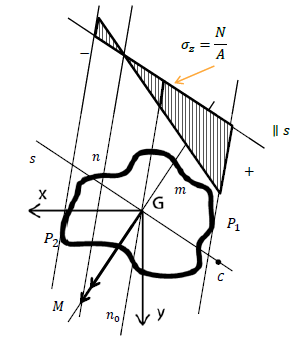
\includegraphics[width=0.5\linewidth]{immagini/screenshot008}
     		\label{fig:screenshot008}
     	\end{figure}
     	   	
     	In pratica la percentuale di rottura è l'integrale della coda della gaussiana della funzione margine di sicurezza sotto lo zero, mentre la percentuale di sopravvivenza sarà il complementare ad uno della rottura, l'area sottesa da tutto il resto della curva. 
     	
     	Con il grafico qui sotto riportato basterà entrare con il numero di deviazioni standard da voler considerare e si uscirà con il relativo valore di affidabilità. 
     	
     	\begin{figure}[H]
     		\centering
     		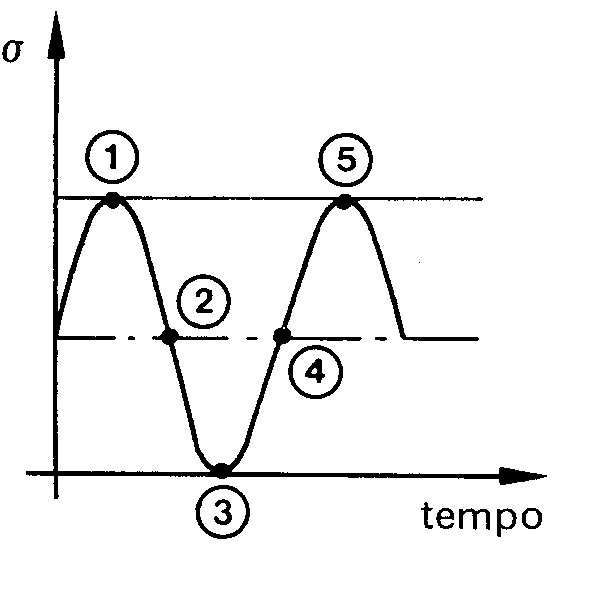
\includegraphics[width=0.75\linewidth]{immagini/screenshot009}
     		\label{fig:screenshot009}
     	\end{figure}
     	
     	Per effettuare un calcolo di progettazione usando gli strumenti probabilistici è necessario conoscere il più possibile la dispersione vera dei valori in esame, è inutile approcciare statisticamente una verifica di resistenza se non si ha una corretta stima della dispersione dei dati e questo non si può non svolgere se non raccogliendo dati sperimentali o facendo campionamenti dei componenti in esercizio: più dati sperimentali si avranno migliore sarà l'affidabilità dello strumento.
     		
     	Matematicamente l'affidabilità si può studiare attraverso una distribuzione normalizzata, e quindi con una variabile normalizzata. 
     	
     	La grandezza margine di sicurezza $z = x - y$ la si caratterizza con un valore medio, questo differenza tra i valori medi, ed una deviazione standard pari alla radice quadrata della somma dei quadrati, in formule: 
     	\[\mu_z = \mu_x - \mu_y \hspace{1cm} \sigma_z = \sqrt{\sigma_x^2 + \sigma_y^2}\]
     	Si può definire un margine di sicurezza affidabilistico $ SM $ \textit{Safety Margin} come il rapporto fra il valore medio e la deviazione standard della grandezza $z$:
     	\[SM = {\mu_z\over\sigma_z} = \dfrac{\mu_x - \mu_y}{ \sqrt{\sigma_x^2 + \sigma_y^2}}\]
     	\begin{figure}[H]
     		\centering
     		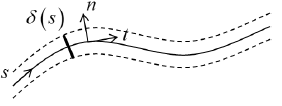
\includegraphics[width=0.5\linewidth]{immagini/screenshot012}
     		\label{fig:screenshot012}
     	\end{figure}     	
     	La probabilità di rottura $P_R$ quindi è la probabilità che la tensione sia maggiore della resistenza, ovvero che la grandezza $z$ sia inferiore allo zero, la probabilità di sopravvivenza del componente $ R $ \textit{reliability} sarà invece il complementare alla probabilità di rottura:
     	\[ \begin{cases}
     		P_R & = P(y>x) = P(z<0) \\
     		R & = P(x>y) = 1 - P_R
     	\end{cases} \]     	
     	Spesso anziché utilizzare il termine "margine di sicurezza $z$" si preferisce usare una distribuzione standardizzata, ovvero:
     	\[\mathcal{Z} = {z-\mu_z\over\sigma_z} \]
     	La probabilità di rottura individuata da questa distribuzione normale standardizzata è nient'altro che l'integrale:
     	\[P_R = \int_{-\infty}^{\mathcal{Z}'}{1\over\sqrt{2\pi}}e^{\mathcal{Z}^2\over 2}dz\]
     	Dove $ \mathcal{Z}' $ è il valore di $ \mathcal{Z} $ associato alla condizione limite, quella in cui la differenza tra resistenza e tensione era nulla: $z =0$, questa condizione porta perciò a definire:
     	\[\mathcal{Z}' = -{\mu_z\over\sigma_z} = -SM \]
     	Poiché la risoluzione dell'integrale è dispendiosa in termini di tempo e risorse, la distribuzione standardizzata permette l'utilizzo di tabelle.
     	
     	\begin{figure}[H]
     		\centering
     		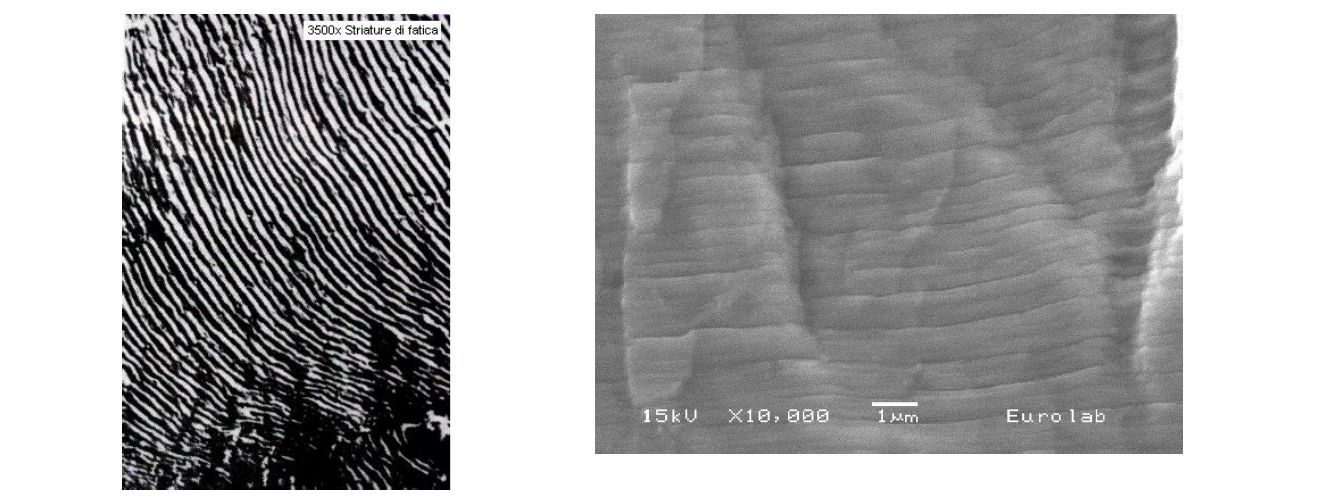
\includegraphics[width=0.7\linewidth]{immagini/screenshot010}
     		\label{fig:screenshot010}
     	\end{figure}
     	    	
     	\textbf{Esempio} \newline 
     \begin{figure}[H]
     	\centering
     	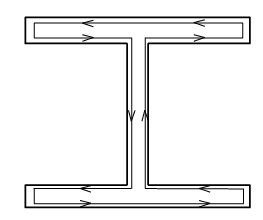
\includegraphics[width=0.5\linewidth]{immagini/screenshot011}
     	\label{fig:screenshot011}
     \end{figure}
     
     	
     	In QUESTO caso $y$ è la resistenza del materiale mentre $x$ è la tensione effettiva sul materiale. 
     	
     	Quest'ultima è caratterizzata dall'avere mediamente un fattore di sicurezza superiore all'unità ma una dispersione più ampia, ha una campana più bassa e più larga rispetto all'altra. 
     	
     	La distribuzione $z$, differenza tra questi valori, individua una probabilità di rottura del componente molto alta, l'area al di sotto dello $ 0 $ è molto ampia, ma come si quantifica? 
     	
     	La condizione limite è quando \(z = 0 \Rightarrow \mathcal{Z}' = -{\mu_z\over\sigma_z} = -1\) per trovare la probabilità di rottura sarà allora necessario effettuare l'integrale tra $-\infty$ e $ -1 $ della distribuzione di Gauss standardizzata. 
     	
     	Attraverso tabella, entrando con un valore di $z = \mathcal{Z}'$ in colonna, si uscirà con un valore di probabilità associato alla probabilità di rottura del componente, in questo caso, entrando con:
     	\[z = \mathcal{Z}' = - 1 \Rightarrow P_R = 16\% \hspace{1cm} R = 84\%\] 
     	
     	Ora, cosa succede se a parità di valori medi si fosse in grado di ridurre la dispersione, diminuendo quindi le deviazioni standard magari di un fattore due, dimezzandola? 
     	\[\begin{matrix}
     		\mu_x = 300 & \mu_y = 400 & \mu_z = 100 \\
     		\sigma_x = 40 & \sigma_y = 30 & \sigma_z = 50 
     	\end{matrix}\]
     	La condizione limite è ora quando \(z = 0 \Rightarrow \mathcal{Z}' = -{\mu_z\over\sigma_z} = -2\),  per cui in questo caso, entrando con:
     	\[z = \mathcal{Z}' = - 2 \Rightarrow P_R = 2.3\% \hspace{1cm} R = 97.7\%\]
     	Qual è il risvolto della medaglia? La riduzione della dispersione dei dati è costoso, si deve lavorare sui processi di produzione, di verifica, di realizzazione, di qualità... 
     	
     
	     
	     
		
		
		
		 
		
		
		
		
	
 		
 		
 		
 		
 		
 		
 		
 		
	 	
	 	
	 	
	 	
	 	
	 	
	 	
		 
		 
		 
	\newpage
	{\Large \textbf{NOTE}}
%	\vfill
%\begin{tcolorbox}[height=4.5cm]
%	This box has a height of 4.5cm.
%\end{tcolorbox}

%DA DECOMMENTARE PER AVERE LA VERSIONE STAMPABILE A DUE PAGINE 	
%	\newpage
%		\null
%		\vfill
%\begin{tcolorbox}[height=4.5cm]
%	This box has a height of 4.5cm.
%\end{tcolorbox}
		\end{adjustwidth}

\end{document}